% =============================================================================
% E-LQTP --- IEEE Internet of Things Journal manuscript
% Driver: inputs every section as a separate .tex file.
% Do not merge with paper/iotj_et_hold.tex (unrelated prior manuscript).
% Numbers from the recorded Western Pacific campaign (Table I).
% =============================================================================
\documentclass[journal]{IEEEtran}

\usepackage{cite}
\usepackage{amsmath,amssymb,amsfonts}
\usepackage{graphicx}
\usepackage{algorithm}
\usepackage{algorithmic}
\usepackage{url}
\usepackage{textcomp}
\usepackage{bm}
\usepackage{dblfloatfix}
\usepackage{float}
\usepackage[section]{placeins}
\renewcommand{\algorithmiccomment}[1]{\hfill//~#1}
\setlength{\textfloatsep}{6pt plus 1pt minus 2pt}
\setlength{\floatsep}{6pt plus 1pt minus 2pt}
\setlength{\intextsep}{6pt plus 1pt minus 2pt}
\setlength{\dbltextfloatsep}{8pt plus 2pt minus 2pt}
\setlength{\dblfloatsep}{6pt plus 1pt minus 2pt}
\setlength{\abovecaptionskip}{3pt}
\setlength{\belowcaptionskip}{0pt}

\hyphenation{Aqua-Sim under-water event-triggered Bellhop E-LQTP LQARP}

\begin{document}

\title{Event-Triggered Link-Quality and Topology Prediction for Mobile
Underwater Wireless Sensor Networks: A Kalman Filter and
Reinforcement Learning Approach}

% IEEE IoT-J author block. First author: Xuefei Ma.
% Corresponding author: Ghulam Ali.
\author{Xuefei~Ma,
        Ghulam~Ali,
        Zhongwei~Shen,
        Insha~Hassan,
        Muhammad~Aon,
        Qingling~Liu,
        Haifeng~Zhu,
        and~Ying~Cui%
\thanks{The authors are with Harbin Engineering University, Harbin
150001, China (e-mail: maxuefei@hrbeu.edu.cn;
ghulamali.cs@gmail.com; shenzhongwei@hrbeu.edu.cn;
inshahassan45@gmail.com; muhammadaoncs29@gmail.com;
liuqingling@hrbeu.edu.cn; zhuhaifeng@hrbeu.edu.cn;
cuiying@hrbeu.edu.cn).}%
\thanks{Corresponding author: Ghulam Ali.}}


\markboth{IEEE Internet of Things Journal}%
{Ma \MakeLowercase{\textit{et al.}}: Event-Triggered Link-Quality and Topology Prediction}

\maketitle

% IEEE IoT-J: one paragraph, 150--250 words, no citations, no displayed math.
\begin{abstract}
Mobile underwater wireless sensor networks must keep link quality
current as vehicles move, yet a fixed neighbor-broadcast timer spends
scarce acoustic airtime while the channel is temporarily stable and
can still miss the instants at which a link-quality forecast has
diverged from the channel. This article presents Event-Triggered
Link-Quality and Topology Prediction (E-LQTP), an extension of the
link-quality-aware routing protocol LQARP. A dual-track extended
Kalman filter maintains a measurement-corrected relative-motion
estimate and a forecast of the same state that receives no
measurement update. Their innovation, gated by a persistence test and
a variance cap, emits a HELLO only when that forecast diverges from a
per-tick channel query. E-LQTP inherits LQARP's multipath channel
model, depth-progressive candidate set, and Bellhop integration; the
Q-learning reward is left unchanged at the validated operating point.
On the same Western Pacific site, with forty relays over six hundred
seconds and five seeds, every protocol reads the same live pose.
E-LQTP then matches LQARP's packet delivery, hops, delay, and energy
per data bit, while cutting control traffic to one-third of a
five-second HELLO grid under two-metre-per-second current drift and
to about one-half under a Rankine eddy. Additive predictive reward
terms do not improve the data plane. The control-plane gain is the
event-triggered HELLO under that shared pose, with the reward left
unchanged.
\end{abstract}

\begin{IEEEkeywords}
Event-triggered communication, extended Kalman filter (EKF), link
quality-aware routing, mobile underwater wireless sensor network (UWSN),
Q-learning, underwater acoustic channel.
\end{IEEEkeywords}

\noindent\textbf{Note to Practitioners:}
A mobile AUV mesh that copies a fixed HELLO timer spends acoustic
airtime on a schedule that ignores whether a link-quality forecast
has diverged from the channel.
E-LQTP keeps LQARP's Bellhop lookup, depth-progressive candidate
set, and Q-learning reward, and fires a $400$-bit HELLO only on a
rising edge of a persistence-gated dual-track innovation.
On the Western Pacific site ($N=40$), with every protocol reading
the same live pose, the validated point (trigger on,
$\beta_1=\beta_2=0$) matches LQARP's data plane while cutting
control traffic to $0.33\times$ a $5\,\mathrm{s}$ grid under
$2\,\mathrm{m/s}$ drift and to $0.51\times$ under a Rankine eddy.
Leave the reward weights at zero.
Energy per bit follows LQARP and excludes HELLO joules; those joules
are reported as control overhead.

\section{Introduction}
\label{sec:intro}
\IEEEPARstart{T}{he} Internet of Underwater Things (IoUT) deploys
acoustic multi-hop meshes for environmental observation, resource
exploration, and maritime awareness
\cite{gupta2024uwsn,gola2023taxonomy,saleem2024ai,jiang2023orsurvey}.
Underwater wireless sensor networks (UWSNs) must route under scarce
bandwidth, long delay, and a time-varying multipath channel
\cite{gupta2024uwsn,saleem2024ai,zhu2024trustcomst}.
An increasingly important case is the \emph{mobile} UWSN, in which
autonomous underwater vehicles (AUVs) and unmanned surface vehicles
(USVs) assist monitoring, adaptive sampling, and mobile relay meshes
\cite{gola2023taxonomy,wang2024lgdqn,liu2025mdqn,lu2025wper}.
There the static or moored-relay assumption common in prior routing
work---including LQARP---breaks down, because relative motion
continuously reshapes geometry and instantaneous link quality
\cite{liu2026lqarp,xu2025stgr}.

Routing under mobility is not new, yet two threads remain poorly
aligned with the control-plane cost of keeping link-quality state
accurate while vehicles move.
First, Q-learning and multi-agent reinforcement-learning UWSN
protocols typically assume that neighbor and link state can be
refreshed by periodic beaconing, or they omit an explicit
relative-motion model that would tell a node \emph{when} advertised
link state has become stale
\cite{nandyala2023qtar,zhang2025saqr,liu2024clorP,xu2025stgr,mohanraju2025adrp}.
Periodic HELLO traffic then consumes scarce acoustic bandwidth even
while the channel is temporarily stable.
Second, event-triggered Kalman filtering now schedules filter packets
for IoUT target tracking and remote estimation
\cite{li2026dse,priel2023consensus,sebastian2024eco,deng2023auto},
Kalman SNR prediction is used to adapt a modem
\cite{busacca2024snr}, and event beacons appear in underwater named
data networking \cite{wang2024push,li2024recar}.
Those designs schedule tracking packets, modem updates, or
named-data events.
The subsections below identify which of them, if any, already fire a
routing HELLO from an SNR forecast that is withheld from the
per-tick channel query.
Motivated by these challenges, we review existing
reinforcement-learning underwater routing and event-triggered
estimation, and identify why neither, on its own, resolves that
control-overhead cost.

\subsection{Related Work}
E-LQTP inherits LQARP's multipath channel model, candidate-set
construction, and Bellhop/Aqua-Sim integration unmodified, so this
section does not reopen the simulation-tool argument treated in that
work \cite{liu2026lqarp}.
The subsections that follow isolate the gaps that mobility introduces
on top of that foundation.

\subsubsection{Reinforcement-Learning UWSN Routing}
Nandyala, Kim, and Cho propose QTAR, a Q-learning topology-aware
protocol that selects a next-forwarder from a topology-constrained
candidate set and uses implicit cut-vertex recognition to avoid
energy-wasting detours \cite{nandyala2023qtar}.
Zhang, Chen, and Xie later add service-aware rewards and a holding
time for opportunistic forwarding (SAQR) \cite{zhang2025saqr}.
Yuan \emph{et~al.} nest Q-learning inside unequal clusters
\cite{yuan2023qhier}, and Wang \emph{et~al.} accelerate Q-table
convergence with a depth-aware opportunistic reward
\cite{wang2023rldepth,wang2024qacc}.
Mohanraju and Lokam replace the tabular update with a deep
Q-network that scores residual energy, depth, and node degree
(ADRP-DQL) \cite{mohanraju2025adrp}.
Wang \emph{et~al.} further split the reward by value of information
so that urgent and delay-tolerant packets share the same MARL
forwarder (MARV) \cite{wang2024marv}.
Liu \emph{et~al.} design CLORP, coupling multi-agent reinforcement
learning with opportunistic forwarding and an adaptive learning rate
\cite{liu2024clorP}.
Xu \emph{et~al.} introduce STGR for multi-UUV meshes: a distributed
spatial-temporal graph records neighbor relations, link quality, and
connectivity duration over periodic intervals, and Q-learning then
selects a forwarder on that graph \cite{xu2025stgr}.
He \emph{et~al.} fold a trust score into the same opportunistic
Q-learning loop so that malicious or unstable relays are down-ranked
\cite{he2025trust}.
Li \emph{et~al.} assist the Q-update from an SDN controller
(SDN-QLTR) \cite{li2024sdnqltr}.
LQARP itself folds Bellhop SNR, residual energy, delay, and neighbor
count into a Q-learning reward on a stationary Western Pacific mesh
\cite{liu2026lqarp}.
Its data plane is the parent of E-LQTP; it does not address when a
mobile node must re-advertise that reward state.
Li, Wu, Zhu, and Ren come closest to the control rule studied here.
Their Q-learning link-aware protocol predicts neighbor motion with an
extended Kalman filter and sets the HELLO period to a fraction of the
shortest predicted link expiration time,
$T_H(N_i)=\tau\min_j T_{\mathrm{LET}}(N_i,N_j)$ with
$\tau\in(0,1)$ \cite{li2025qlar}.
High relative motion shortens the period and low relative motion
lengthens it, and the same expiration time enters the reward through
an entropy-weight combination.
That rule already withholds some beacon traffic while a
geometrically predicted link is expected to survive.
It remains a periodic timer scaled by link lifetime, and it spends
the predicted lifetime inside the reward.
It does not compare an SNR forecast, withheld from measurement
updates since the last velocity write, with a channel query taken
every tick.
In the other protocols above, neighbor perception remains a periodic
exchange or a timer-rebuilt graph.

\subsubsection{Mobility-Aware and AUV-Assisted Collection}
Wang \emph{et~al.} plan cooperative multi-AUV collection with
local--global deep Q-learning and a separate emergency multi-hop
route \cite{wang2024lgdqn}.
Liu \emph{et~al.} and Lu and Zuo treat the AUV as a path-planning
agent whose reward includes ocean current and communication capacity
\cite{liu2025mdqn,lu2025wper}.
Nandyala and Cho dispatch an AUV to prevent isolated sub-networks
once isolation is declared \cite{nandyala2025isolated}.
Jiang \emph{et~al.} opportunistically switch between acoustic and
radio hops in a cooperative surface--subsurface mesh
\cite{jiang2023hybrid}.
Yuan \emph{et~al.} jointly optimize multi-objective routes and a
centralized cross-layer schedule of power, links, and next hops
\cite{yuan2024multiobj,yuan2024crosslayer}.
In all of these designs the vehicle is a collector, a repair asset,
or a radio relay---not a source of estimated relative motion that
could gate neighbor broadcasts before advertised SNR goes stale.

\subsubsection{Opportunistic, Clustered, and Information-Centric Forwarding}
Jiang, Han, and Lin survey opportunistic IoUT routing and note that
candidate-set maintenance is still a periodic control cost
\cite{jiang2023orsurvey}.
Zhu \emph{et~al.} cluster relays and predict voids with a Markov
model (RCRP) \cite{zhu2024rcrp}, later adding a GMM--HMM--LSTM
adaptive route \cite{zhu2024gmmhmm}; a companion COMST article
gives trust-management guidelines for the same setting
\cite{zhu2024trustcomst}.
Lee \emph{et~al.} form energy-efficient clusters with a fire-hawk
optimizer and still emit periodic HELLO packets during neighbor
discovery \cite{lee2025fho}.
Wang \emph{et~al.} replace a passive interest with an actively
forwarded beacon when a critical event occurs in underwater named
data networking \cite{wang2024push}.
Li \emph{et~al.} avoid collisions among those NDN paths (RECAR)
\cite{li2024recar}, and Wang, Lu, and Gao cache push and pull
modes for information-centric underwater IoT
\cite{wang2025reliable}.
Zhao \emph{et~al.} add time-reversal opportunistic forwarding
\cite{zhao2026trclor}.
Tian \emph{et~al.} hide source location behind layered candidates
\cite{tian2023lslpr}, and Yuan \emph{et~al.} validate a
source-based disjoint multipath protocol in Zhoushan sea trials
\cite{yuan2024multipath}.
Those beacons and candidate sets are application-level or
path-diversity events, not a routing HELLO tied to a
relative-motion residual.

\subsubsection{Event-Triggered Estimation and Channel Prediction}
Priel and Zelazo develop event-triggered consensus Kalman filtering
for time-varying networks with intermittent observations
\cite{priel2023consensus}.
Sebasti\'{a}n \emph{et~al.} certify an event-triggered distributed
Kalman filter under unknown correlations \cite{sebastian2024eco}.
Deng and Xiong infer the remote state when the trigger decision
itself is hidden \cite{deng2023auto,deng2024lcsys}, and Zhong
\emph{et~al.} schedule multiple sensors over packet-dropping links
\cite{zhong2024tsp}.
Closest in venue and in the use of a predicted state as the trigger
reference, Li~\emph{et~al.} design two media-specific event triggers
for consensus Kalman filtering over a hybrid IoUT
\cite{li2026dse}.
When a surface node does not transmit, neighbors propagate the last
broadcast through the Kalman predict step, yielding a predicted
information pair against which the next innovation is tested.
That construction is the nearest cousin of the forecast track in
Section~III: both ask what a neighbor still believes after a missed
transmission.
Li~\emph{et~al.} reset the predicted information pair when a packet
arrives.
The forecast in Section~III is reset when the local broadcast flag
is high, by copying the neighbor's current odometry, and the copy is
not a demodulated packet.
The scheduled object in \cite{li2026dse} remains a filter packet for
AUV \emph{tracking}, rather than a HELLO that refreshes advertised
link quality for Q-learning forwarding.

A related physical-layer thread predicts SNR itself rather than
scheduling a packet.
Busacca~\emph{et~al.} compare $N$-state Markov and hidden-Markov
models with a scalar Kalman filter on NATO LOON21 traces
\cite{busacca2024snr}.
On those fixed, shallow links the Kalman mean absolute SNR error is
$4.81\,\mathrm{dB}$ on the 11~November 2021 traces,
$3.47\,\mathrm{dB}$ when that model is tested on 14~November, and
$3.24\,\mathrm{dB}$ when it is tested on 18~November.
The $2\,\mathrm{dB}$ cap in Section~III is a design choice of this
paper, placed below those three fixed-link errors.
Busacca~\emph{et~al.} use the filter to adapt a constellation;
they do not prescribe a HELLO threshold.
The dual-track EKF below is a staleness detector for HELLO, not an
SNR-RMSE competitor.

Overall, two issues remain open.
First, the reinforcement-learning and opportunistic protocols
reviewed above, other than QLAR, keep link state current by periodic
beaconing or by a timer-rebuilt graph
\cite{nandyala2023qtar,xu2025stgr,liu2026lqarp,zhu2024rcrp}.
QLAR does test predicted link lifetime, and it uses that lifetime
both to scale a periodic HELLO and to shape the reward
\cite{li2025qlar}.
Second, event-triggered Kalman filtering schedules filter packets
for IoUT tracking and remote estimation
\cite{li2026dse,sebastian2024eco,zhong2024tsp}, Kalman SNR
prediction adapts a modem \cite{busacca2024snr}, and event beacons
appear in UNDN \cite{wang2024push}.
None of those three threads schedules a routing HELLO from the
divergence between an SNR forecast that receives no measurement
update and a channel measurement taken at every tick.

\subsection{Contributions}
The contributions of this article are summarized as follows.

\begin{enumerate}
\item To answer the two gaps jointly, we design a dual-track
relative-motion estimator---a measurement-corrected track and a
forecast track that receives no measurement update---so that an event trigger can be
computed even though the channel-quality measurement is available
every tick.
Its innovation, gated by a persistence condition and a
variance-capped threshold, decides when a node broadcasts the
velocity copy that resets the forecast.
The resulting Event-Triggered Link-Quality and Topology Prediction
protocol (E-LQTP) replaces periodic HELLO traffic with that
motion-aware copy.

\item We investigate whether the same relative-motion estimate can
directly inform the Q-learning reward through a predictive
link-quality term and a drift-aware forwarding term, and we
characterize---rather than tune away---the conditions under which
this does \emph{not} improve routing: a bit-error-rate floor that
creates a scale mismatch with an additive prediction penalty, and a
radial-velocity sign persistence shorter than one hop's transit
time.
This is reported as a scoped, evidence-based negative result.
\end{enumerate}

\subsection{Paper Organization}
The rest of this article is organized as follows.
Section~II introduces the extended system model of a mobile UWSN
under uniform current drift and Rankine-vortex eddy motion.
Section~III details the design of E-LQTP, including the dual-track
extended Kalman filter, the persistence-gated event trigger, and the
scoped Q-learning reward terms.
Section~IV presents simulation results on the Western Pacific site
for both mobile scenarios.
Section~V concludes.

\section{Preliminaries}
\label{sec:prelim}

This section states the mobile-UWSN architecture and the acoustic,
multipath, noise, and Q-learning objects that E-LQTP inherits from
LQARP \cite{liu2026lqarp}.
The inherited objects are restated so that the dual-track estimator
of Section~\ref{sec:design} can be written against a closed system
model; no new channel or learning contribution is claimed.
Subsection~\ref{sec:prelim:est} isolates the estimation problem that
mobility adds on top of that foundation.

\subsection{Network Architecture}
\label{sec:prelim:arch}
\begin{figure*}[!t]
\centering
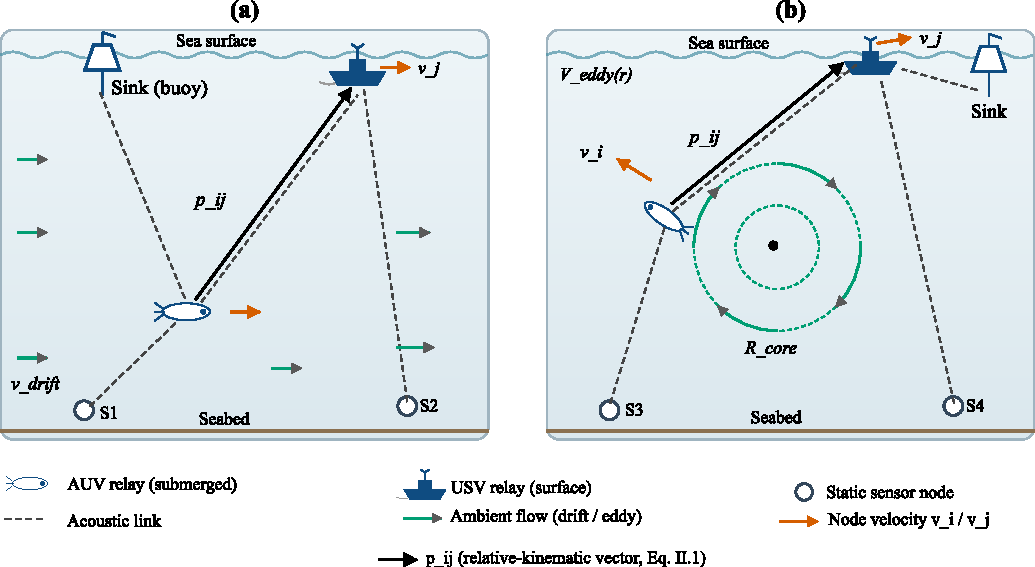
\includegraphics[width=\textwidth]{elqtp_figs/fig1_network_architecture}
\caption{Mobile UWSN. (a)~Shared current. (b)~Rankine eddy.
Solid: relative kinematic vector $p_{ij}$. Dashed: acoustic link.}
\label{fig:network_architecture}
\end{figure*}

The network is a single-sink acoustic mesh of $N$ autonomous
underwater vehicles (AUVs) and one unmanned surface vehicle (USV)
sink, deployed in a
$L\times L\times H=6\,\mathrm{km}\times 6\,\mathrm{km}\times
500\,\mathrm{m}$ Western Pacific water column
(Fig.~\ref{fig:network_architecture}).
The sink sits at the horizontal centroid with kinematic depth
$z_{\mathrm{sink}}=5\,\mathrm{m}$, so that it is uniquely shallowest
for the depth-progressive candidate filter of
Section~\ref{sec:prelim:q}.
Its acoustic query depth is independent of that kinematic depth and
is set to the Bellhop source-depth slice $z_{\mathrm{ac}}=50\,\mathrm{m}$
(a towed or hull-offset transducer).
Each AUV $s_i$ has kinematic state
$(p_i,\dot{p}_i)\in\mathbb{R}^3\times\mathbb{R}^3$, residual energy
$E_{s_i}$, and a feasible-neighbor count $\mathrm{number}_{s_i}$.
Relays are placed uniformly in
$[0,L]^2\times[10,H]$ with a $1\,\mathrm{m}$ three-dimensional
separation floor.
The sink does not generate data.
Every AUV emits a data packet of $l=400\,\mathrm{bit}$ every
$30\,\mathrm{s}$.

Two mobility fields are used in evaluation
(Fig.~\ref{fig:network_architecture}) and are drawn at $N=40$ in
Fig.~\ref{fig:mobility_fields}.
Scenario~I is the stationary identity:
$\dot{p}_i\equiv 0$.
Scenario~II is a shared horizontal current
$\dot{p}_i(t)=v_{\mathrm{cmd},i}+v_{\mathrm{drift}}$ with
$v_{\mathrm{cmd},i}=0$ and $\dot{p}_{\mathrm{sink}}=0$, so that
AUV--AUV relative velocity is identically zero and the only
persistent range-rate is AUV-to-sink.
Scenario~III replaces the uniform current with a counterclockwise
Rankine eddy centered on the sink plus an independent horizontal
Gauss--Markov fluctuation, so that AUV--AUV $v_{\mathrm{rel}}$ is
nonzero.
A relay that leaves the valid horizontal envelope is removed;
in-flight packets at that node fail as envelope-exit losses, not voids.
Vertical current is not modelled: a $1\,\mathrm{m/s}$ vertical
component would empty the $500\,\mathrm{m}$ column in a few hundred
seconds.

\subsection{Underwater Acoustic Channel}
\label{sec:prelim:urick}
Instantaneous link quality is the sonar-equation SNR on a
precomputed Bellhop field, inherited from LQARP
\cite{liu2026lqarp}.
For a transmitter--receiver pair $(s_i,s_j)$,
\begin{equation}
\label{eq:snr}
\mathrm{SNR}(s_i,s_j)
= \mathrm{SL}-\mathrm{TL}(r_H,z_q)-\mathrm{NL}+\mathrm{DI},
\end{equation}
where $\mathrm{SL}=175\,\mathrm{dB}$ re $1\,\mu\mathrm{Pa}@1\,\mathrm{m}$
is the source level, $\mathrm{DI}=0\,\mathrm{dB}$ is the
omnidirectional directivity index, and $\mathrm{NL}$ is the
band-integrated Wenz level of Section~\ref{sec:prelim:noise}.
Horizontal range $r_H=\|(x_i-x_j,y_i-y_j)\|$ and query depth
$z_q=\max(z_j^{\mathrm{ac}},5\,\mathrm{m})$ index a January
World Ocean Atlas 2023 / GEBCO cell at
$20.125^\circ\mathrm{N}$, $124.125^\circ\mathrm{E}$
(seafloor $5524\,\mathrm{m}$, source depth $50\,\mathrm{m}$,
carrier $24\,\mathrm{kHz}$, integration band $B=2\,\mathrm{kHz}$).
Transmission loss is the sonar-equation column of that grid,
\begin{equation}
\label{eq:tl}
\mathrm{TL}(r_H,z_q)=-10\log_{10}\bar{G}(r_H,z_q),
\end{equation}
with $\bar{G}$ the in-band power average of the equivalent transfer
function reconstructed from Bellhop eigenrays (geometric spreading
with $\kappa=2$ and Thorp absorption as in LQARP
\cite{liu2026lqarp}; Bellhop amplitudes are not reused, so spreading
and absorption are not double-counted).
A lookup that is non-finite is treated as a failed link:
$\mathrm{SNR}\ge\mathrm{SNR}_{\mathrm{th}}=8.68\,\mathrm{dB}$ is
reception, and any non-finite or sub-threshold value is a failed link.
The January $50\,\mathrm{m}$ crossing range at that threshold is
$r_{\mathrm{range}}=5125\,\mathrm{m}$.
Every protocol variant---LQARP, E-LQTP, the RLOR-inspired baseline,
and the Fixed-Periodic ablation---uses the same Bellhop lookup for
every SNR decision \cite{liu2026lqarp}.

\subsection{Multipath Representation}
\label{sec:prelim:mp}
The channel is frequency-selective on this site.
Water-column delay spread of about $3\,\mathrm{ms}$ at $1\,\mathrm{km}$
sets a coherence bandwidth of a few hundred hertz, much narrower
than $B=2\,\mathrm{kHz}$.
The scalar used by routing is therefore the $2\,\mathrm{kHz}$
power average $\bar{G}$, not a single-frequency coherent snapshot.
That average is the LQARP-style link budget; it does not resolve
fast fading, and the median pre-filter of
Section~\ref{sec:design:ekf} is not claimed to do so either.
Out-of-envelope (range, depth) cells are stored as non-finite and
are rejected by the reception gate rather than interpolated.

\subsection{Ambient Noise}
\label{sec:prelim:noise}
Ambient noise follows the four-component Wenz model inherited from
LQARP \cite{liu2026lqarp} at shipping factor $s=0.2$ and wind
$w=2.0\,\mathrm{m/s}$ (assumed, not taken from WOA/GEBCO).
The band-integrated level over $23$--$25\,\mathrm{kHz}$ is
$\mathrm{NL}=65.77\,\mathrm{dB}$ re $1\,\mu\mathrm{Pa}$.
At $24\,\mathrm{kHz}$ the spectral densities (dB re
$1\,\mu\mathrm{Pa}^2/\mathrm{Hz}$) are turbulence $-24.4$,
shipping $-13.0$, wave $32.7$, and thermal $12.6$; wind and thermal
terms dominate.
$\mathrm{NL}$ is constant on the grid; motion enters
\eqref{eq:snr} only through $\mathrm{TL}(r_H,z_q)$.

\subsection{Q-learning Routing}
\label{sec:prelim:q}
LQARP treats each node $s_i$ as a Q-learning agent
\cite{liu2026lqarp} on the MDP $(S,A,P,R)$.
The action $a_j$ selects neighbor $s_j$ as next hop.
A neighbor is a candidate only if it lies in all three of
\begin{align}
\label{eq:cand}
N_{\mathrm{range}}(s_i)
&= \{s_j:d(s_i,s_j)<r_{\mathrm{range}}\},\nonumber\\
N_{\mathrm{SNR}}(s_i)
&= \{s_j:\mathrm{SNR}(s_i,s_j)>\mathrm{SNR}_{\mathrm{th}},\,j\neq i\},\nonumber\\
N_{\mathrm{depth}}(s_i)
&= \{s_j:\mathrm{depth}_{s_i}-\mathrm{depth}_{s_j}>0,\,j\neq i\},
\end{align}
so that
$I(s_i)=N_{\mathrm{range}}(s_i)\cap N_{\mathrm{SNR}}(s_i)\cap
N_{\mathrm{depth}}(s_i)$ and $A=I(s_i)$.
The reward on a feasible action is
\begin{equation}
\label{eq:reward_lqarp}
R^{a_j}_{s_i,s_j}
= \frac{c_{\mathrm{ene}}(s_j)\,c_{\mathrm{del}}(s_i,s_j)\,
c_{\mathrm{nei}}(s_j)}{c_{\mathrm{lin}}(s_i,s_j)},
\end{equation}
with
\begin{align}
\label{eq:factors}
c_{\mathrm{lin}}(s_i,s_j)
&= \ln\!\bigl(1/P_{\mathrm{succ}}(s_i,s_j)\bigr),\nonumber\\
P_{\mathrm{succ}}
&= (1-p_e)^l,\nonumber\\
c_{\mathrm{ene}}(s_j)
&= (2/\pi)\arctan\bigl((E_{s_j}-E_{\mathrm{avg}})/E_{\mathrm{ini}}\bigr),\nonumber\\
c_{\mathrm{del}}(s_i,s_j)
&= (E_{s_j}/E_{\mathrm{ini}})\,
(\mathrm{depth}_{s_i}-\mathrm{depth}_{s_j}),\nonumber\\
c_{\mathrm{nei}}(s_j)
&= \exp(\mathrm{number}_{s_j}).
\end{align}
$p_e$ is the $M=2$ (BPSK) OFDM bit-error expression of LQARP
Eq.~34, floored at $p_e=\max(p_e^{\mathrm{AWGN}},10^{-9})$ so that
$c_{\mathrm{lin}}$ remains finite on the high-SNR plateau that is
typical at short range on this grid
($c_{\mathrm{lin}}\approx 4\times 10^{-7}$ for $l=400$).
$E_{\mathrm{avg}}$ is the mean residual energy over $I(s_i)$, not
the global mean; $\mathrm{number}_{s_j}=|I(s_j)|$, and
$c_{\mathrm{nei}}=1$ when $s_j$ has no onward candidate.
The temporal-difference update is
\begin{equation}
\label{eq:q}
Q(s_i,a_j)
\leftarrow (1-\alpha)Q(s_i,a_j)
+\alpha\Bigl[R^{a_j}_{s_i,s_j}
+\gamma\max_{a\in I(s_j)}Q(s_j,a)\Bigr],
\end{equation}
with $\alpha=0.9$, $\gamma=0.8$, and
$s_i.\mathrm{NextHop}=\arg\max_{a_j\in I(s_i)}Q(s_i,a_j)$.
Q-values start at zero.

When $I(s_i)=\emptyset$ at a non-sink node, LQARP (and E-LQTP)
compute a relaxed detour set
$D(s_i)=N_{\mathrm{range}}(s_i)\cap N_{\mathrm{SNR}}(s_i)$
and keep only two-hop-viable, unvisited members, with a cap of
three detour hops per packet.
That mechanism is a bounded reading of LQARP's qualitative
two-hop remark, applied identically to LQARP, E-LQTP, and
Fixed-Periodic; it is not a new contribution.

\subsection{Relative-Motion Estimation}
\label{sec:prelim:est}
LQARP evaluates $I(s_i)$ and the four reward factors from neighbor
state.
Under mobility a deployed node must decide when to re-advertise
velocity and residual energy, because a periodic HELLO spends
airtime while the acoustic link is still accurate and a silent node
would leave that advertisement unchanged.
In the campaign reported here, no neighbor table ages.
At every forwarding decision and every EKF tick, LQARP, E-LQTP, the
RLOR-inspired baseline, and Fixed-Periodic read the simulator's
current pose together with a fresh Bellhop sample.
That sample is the ground-truth channel query used for reception,
available at every simulation tick $dt=1\,\mathrm{s}$.
The HELLO of Section~\ref{sec:design:ekf} is the charged velocity
copy that resets the forecast.
$I(s_i)$ is taken from the live pose.
Ordinary event-triggered Kalman filtering
\cite{priel2023consensus,li2026dse,sebastian2024eco,deng2023auto,zhong2024tsp}
tests an innovation $z_k-h(\hat{x}_{k|k-1})$ and therefore
\emph{cannot} accumulate staleness here: the measurement-corrected
track heals the only observable dimension (horizontal range) on
every tick, whether or not a HELLO has ever been heard.
The one-step Kalman innovation $e_k$ is consequently a noise
residual, not a ZOH-velocity residual, for any finite threshold.
That is why E-LQTP keeps a second forecast track, propagated
without a measurement update, and triggers on the
forecast-versus-truth innovation of
Section~\ref{sec:design:ekf}, following the predicted-information
idea of Li~\emph{et~al.} \cite{li2026dse} but scheduling a routing
HELLO rather than a tracking packet.
The $2\,\mathrm{dB}$ cap on that trigger threshold is a choice of
this paper.
It lies below the LOON21 Kalman mean absolute SNR errors of
Busacca~\emph{et~al.}, which are $4.81$, $3.47$, and
$3.24\,\mathrm{dB}$ on the three tests cited in
Section~\ref{sec:intro} \cite{busacca2024snr}.
The filter is a staleness detector for HELLO, not an SNR-RMSE
competitor.
\FloatBarrier

\section{E-LQTP Design}
\label{sec:design}

E-LQTP is LQARP plus a dual-track relative-motion estimator, a
persistence-gated HELLO, an optional pair of reward modifiers, and a
stability pre-filter on the candidate set.
The validated operating point uses the estimator and the trigger and
sets the reward modifiers to zero.
Fig.~\ref{fig:mechanism} is the per-tick mechanism;
Algorithm~\ref{alg:elqtp} is the same loop in the equation-referenced
form of LQARP's Algorithm~1 \cite{liu2026lqarp}.
\begin{figure*}[!t]
\centering
\includegraphics[width=\textwidth]{elqtp_figs/fig_mechanism}
\caption{E-LQTP per-tick mechanism.
(a)~Discovery: sensing, dual-track estimation, event trigger, and
rising-edge HELLO.
(b)~Forwarding at $\beta_1=\beta_2=0$, inherited from LQARP.}
\label{fig:mechanism}
\end{figure*}


\subsection{Kinematic State}
\label{sec:design:kin}
For each directed pair $(s_i,s_j)$,
\begin{align}
\label{eq:rel}
p_{ij}(t)&=p_i(t)-p_j(t),\nonumber\\
\dot{p}_{ij}(t)&=\dot{p}_i(t)-\dot{p}_j(t),\nonumber\\
v_{\mathrm{rel}}(i,j)
&= \bigl(\dot{p}_{ij}\cdot p_{ij}\bigr)/\|p_{ij}\|.
\end{align}
Negative $v_{\mathrm{rel}}$ is closing range.
Own velocity $\dot{p}_i$ is odometry and is known exactly.
Neighbor velocity $\dot{p}_j$ is a zero-order hold.
Before any hold has been written the hold is $(0,0,0)$.
Under the shared current of Scenario~II that initialization assigns
pair $(i,j)$ the relative velocity $\dot{p}_i$, which is not the
true relative velocity of two relays drifting together.
The assignment is intentional: writing $j$'s true velocity at
$t=0$ would make every AUV--AUV pair a perfect match to the
constant-velocity model and would leave the trigger with no
innovation on those pairs.
On every later tick for which $\mathrm{Broadcast}_k(i,j)=1$,
including ticks on which the flag stays high after the rising edge,
the three velocity components of the corrected track are overwritten
with no blending,
$\hat{x}_{k|k}^{(v)}\leftarrow\dot{p}_i-\dot{p}_j^{\mathrm{live}}$,
and the forecast track is reset to that corrected state.
The optional drift term does not use the initial hold.
Until the first overwrite, $\beta_2$ is omitted and
$c_{\mathrm{drift}}=c_{\mathrm{del}}$.
SNR does not observe the velocity block.
Horizontal range is adjusted only through the predict Jacobian of
Section~\ref{sec:design:ekf}.
The velocity hold is therefore the sole source of $v_{\mathrm{rel}}$
for the optional drift term.

Scenario~II kinematics are
$\dot{p}_i(t)=v_{\mathrm{drift}}^{(0)}$ with
$\|v_{\mathrm{drift}}^{(0)}\|$ swept in
$[0.5,3.5]\,\mathrm{m/s}$ (reported midpoint $2\,\mathrm{m/s}$)
and one horizontal azimuth, drawn once per run and shared by every relay.
Scenario~III uses a Rankine-capped counterclockwise eddy of core
radius $R_{\mathrm{core}}=2000\,\mathrm{m}$ and speed
$V_{\mathrm{eddy}}=2\,\mathrm{m/s}$ centered at $(3000,3000)\,\mathrm{m}$,
\begin{equation}
\label{eq:rankine}
v_\theta(r)=V_{\mathrm{eddy}}\min(r/R_{\mathrm{core}},1),
\end{equation}
plus the discrete Gauss--Markov step
\begin{equation}
\label{eq:gm}
v^i_{k+1}
= \zeta v^i_k + (1-\zeta)\,v_{\mathrm{eddy}}(p_i)
+ \sqrt{1-\zeta^2}\,\sigma\odot w^i_k,
\end{equation}
with $\zeta=0.95$, $dt=1\,\mathrm{s}$,
$\sigma=(1,1,0)\,\mathrm{m/s}$, and $w^i\sim\mathcal{N}(0,I)$.
The zero vertical innovation is a modelling choice: mid-latitude
mesoscale flow at these scales is geostrophic, and a $1\,\mathrm{m/s}$
vertical term would empty the column.
Inside the solid-body core the mean-flow pair difference is
perpendicular to the line of sight; the Gauss--Markov innovation
supplies most of the observable radial projection
(mean $|v_{\mathrm{radial}}|\approx 1.06\,\mathrm{m/s}$ against
mean $|v_{\mathrm{tangential}}|\approx 2.54\,\mathrm{m/s}$ on the
kinematics-only diagnostic).

\subsection{Dual-Track EKF and Event Trigger}
\label{sec:design:ekf}
\begin{figure*}[!t]
\centering
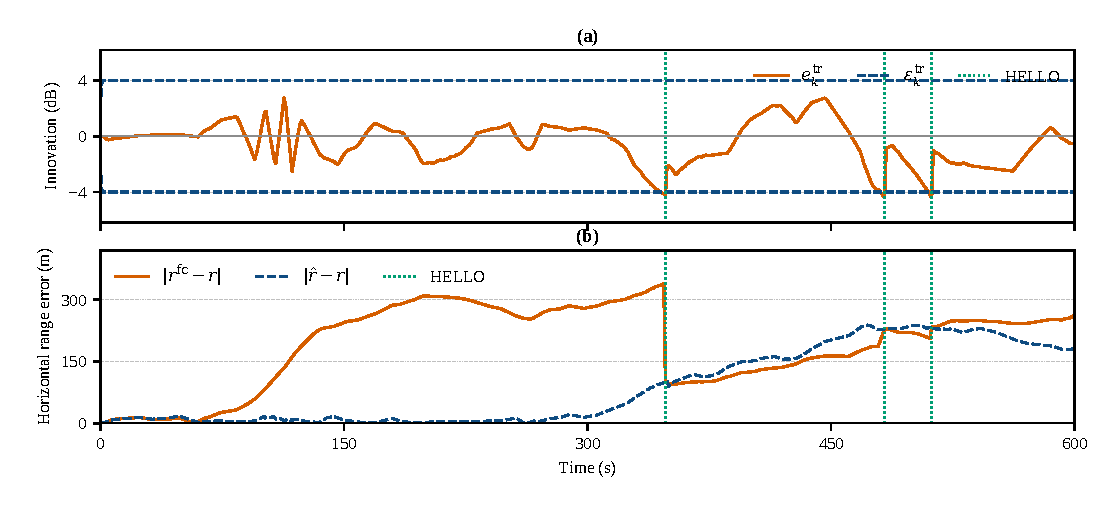
\includegraphics[width=\textwidth]{elqtp_figs/fig7_trigger_trace}
\caption{Dual-track trigger, pair $(1,2)$. (a)~$e_k^{\mathrm{tr}}$
and $\pm\varepsilon_k^{\mathrm{tr}}$. (b)~Range error. HELLOs at
$348$, $483$, $512\,\mathrm{s}$.}
\label{fig:trigger_trace}
\end{figure*}

Each neighbor pair carries a seven-dimensional state
\begin{equation}
\label{eq:state}
x_k=\bigl[p_{ij}^\top,\,\dot{p}_{ij}^\top,\,\mathrm{SNR}_{ij}\bigr]^\top.
\end{equation}
The position--velocity block is constant-velocity,
\begin{equation}
\label{eq:Fkin}
F_{\mathrm{kin}}
=\begin{bmatrix} I_3 & dt\,I_3 \\ 0_3 & I_3 \end{bmatrix},
\end{equation}
and does not carry SNR.
Both tracks apply the same nonlinear predict.
Writing $p^+=p+dt\,\dot{p}$ and
$r_H^+=\|(p_x^+,p_y^+)\|$ for the predicted horizontal range,
with $z_q$ the neighbor's acoustic query depth,
\begin{equation}
\label{eq:forecast}
\begin{aligned}
p^+&=p+dt\,\dot{p},&
\dot{p}^+&=\dot{p},\\
\mathrm{SNR}^+
&=
\begin{cases}
\mathrm{SNR}(r_H^+,z_q), & \text{if the lookup is finite},\\
\mathrm{SNR}^-, & \text{otherwise,}
\end{cases}
\end{aligned}
\end{equation}
The lookup is \eqref{eq:snr}.
An out-of-envelope cell keeps the last finite SNR; it is not
interpolated.
The covariance is propagated by the $7\times 7$ Jacobian $F$ of
\eqref{eq:forecast}: $F=I_7$, the three constant-velocity couplings
are $F_{1,4}=F_{2,5}=F_{3,6}=dt$, the SNR row is replaced rather
than scaled so $F_{7,7}=0$, and the only nonzero SNR--position
entries are the horizontal radial derivatives
\begin{equation*}
F_{7,1}
=\frac{\partial\mathrm{SNR}}{\partial r_H}\frac{p_x^+}{r_H^+},\qquad
F_{7,2}
=\frac{\partial\mathrm{SNR}}{\partial r_H}\frac{p_y^+}{r_H^+}.
\end{equation*}
The range derivative is a central difference with step
$10\,\mathrm{m}$.
Process noise is then added on the diagonal,
$P^+=FPF^\top+Q$, with
$q_{\mathrm{pos}}=1.0$, $q_{\mathrm{vel}}=0.1$, and
$q_{\mathrm{SNR}}=1.0$.
The measurement variance is
$R=r_{\mathrm{meas}}=4.0\,\mathrm{dB}^2$.

Two tracks run in parallel and share \eqref{eq:forecast}.
The \emph{corrected} track $(\hat{x},P)$ also applies a measurement
update.
The raw sample $z_k$ is the Bellhop SNR at the nodes' true current
positions, computed every $dt$ whether or not a packet is heard.
The median $\tilde{z}_k$ is taken over the samples stored for that
pair, at most $W_{\mathrm{mp}}=3$; the first ticks use the shorter
prefix.
The one-step innovation
$e_k=\tilde{z}_k-\hat{x}^{\mathrm{SNR}}_{k|k-1}$
enters the filter and, optionally, $c_{\mathrm{pred}}$.
The update uses $H=[0\,0\,0\,0\,0\,0\,1]$ because the measurement
is the SNR component.
The gain is the corresponding column of $P$,
$K=P_{:,7}/S_k$ with $S_k=P_{7,7}+r_{\mathrm{meas}}$, so the
innovation moves every state component that has covariance with SNR.
Horizontal range is among those components because $F_{7,1}$ and
$F_{7,2}$ couple predicted range into the SNR variance.
The tangential directions and the velocity block are not directly
observed by $H$.
The \emph{forecast} track $(x^{\mathrm{fc}},P^{\mathrm{fc}})$
receives the predict and no measurement update.
It is reset to $(\hat{x}_{k|k},P_{k|k})$ on every tick with
$\mathrm{Broadcast}_k(i,j)=1$, after the corrected-track update,
by the velocity overwrite of Section~\ref{sec:design:kin}.
The trigger innovation uses the raw query against the forecast SNR,
which \eqref{eq:forecast} has just set to the lookup at the
forecast range,
\begin{equation}
\label{eq:etrigger}
e_k^{\mathrm{tr}}
= z_k - \mathrm{SNR}\bigl(r_H(x^{\mathrm{fc}}_k),z_q\bigr).
\end{equation}
A one-step $e_k$ cannot form this residual: the corrected track is
healed every tick, whereas $x^{\mathrm{fc}}$ accumulates the motion
implied by the held velocity.

The corrected-track threshold is left uncapped.
The forecast covariance is not measurement-updated, so
$\varepsilon_0+\lambda\sqrt{S_k^{\mathrm{tr}}}$ would make a
long-silent pair progressively harder to trigger.
The trigger threshold therefore caps the uncertainty term,
\begin{equation}
\label{eq:eps}
\begin{aligned}
\varepsilon_k
&= \varepsilon_0+\lambda\sqrt{S_k},\\
\varepsilon_k^{\mathrm{tr}}
&= \varepsilon_0+\lambda\min\bigl(\sqrt{S_k^{\mathrm{tr}}},
s_{\mathrm{cap}}\bigr),
\end{aligned}
\end{equation}
with $\varepsilon_0=2.0\,\mathrm{dB}$, $\lambda=1$,
$s_{\mathrm{cap}}=\sqrt{r_{\mathrm{meas}}}=2.0\,\mathrm{dB}$,
$S_k=P_{7,7}+r_{\mathrm{meas}}$, and
$S_k^{\mathrm{tr}}=P^{\mathrm{fc}}_{7,7}+r_{\mathrm{meas}}$.
The cap is the design choice identified in
Section~\ref{sec:intro}; it is not taken from
\cite{busacca2024snr}.
A persistence gate with width $W=5$ and fraction $\rho=0.6$ then
sets the flag.
Let $n_k$ be the number of finite trigger samples retained for the
pair, at most $W$.
Until five samples have been stored, $n_k$ is that shorter prefix,
so a single early exceedance has fraction one and can pass
$\rho$.
\begin{equation}
\label{eq:bc}
\begin{aligned}
\mathrm{Broadcast}_k&=1
\quad\text{if }|e_k^{\mathrm{tr}}|\ge\varepsilon_k^{\mathrm{tr}}\\
&\quad\text{and }
\tfrac{1}{n_k}\textstyle\sum_{m\in\mathcal{W}_k}
\mathbf{1}\{|e_m^{\mathrm{tr}}|\ge\varepsilon_m^{\mathrm{tr}}\}\ge\rho,\\
\mathrm{Broadcast}_k&=0
\quad\text{otherwise,}
\end{aligned}
\end{equation}
where $\mathcal{W}_k$ is the retained window.
A non-finite $z_k$ skips the update and forces
$\mathrm{Broadcast}_k=0$.
Node $j$ originates one HELLO on a tick if
$\mathrm{Broadcast}_k(i,j)$ rises for any observer $i$.
Ticks on which the flag merely stays high do not add a further
transmission.
Those ticks do repeat the velocity overwrite and the forecast reset.

Fig.~\ref{fig:trigger_trace} shows the two tracks on
Scenario~III pair $(1,2)$.
Panel~(a) is $e_k^{\mathrm{tr}}$ against
$\pm\varepsilon_k^{\mathrm{tr}}$; the threshold sits at the
$s_{\mathrm{cap}}$ ceiling once forecast variance has grown.
Rising-edge HELLOs occur at $t=348$, $483$, and $512\,\mathrm{s}$.
Panel~(b) is the corresponding horizontal range error.
The forecast range error grows while the flag is low and is reset
when the flag is high.
The corrected range error stays smaller because the per-tick query,
acting through $K$, heals the radial state.
That is the mechanism the control-plane results of
Section~\ref{sec:eval} attribute the overhead reduction to.

\begin{algorithm}[!t]
\caption{E-LQTP: Event-Triggered HELLO and Q-Learning Forwarding}
\label{alg:elqtp}
\begin{algorithmic}[1]
\REQUIRE poses $(p_i,\dot{p}_i)$; hold $\dot{p}_j\leftarrow 0$ until written;
$(\hat{x},P)$, $(x^{\mathrm{fc}},P^{\mathrm{fc}})$
\ENSURE one HELLO per rising node; $s_i.\mathrm{NextHop}$
\STATE {\bfseries Discovery:} dual-track predict \eqref{eq:forecast}
\FOR{each directed pair $(i,j)$}
  \STATE Predict both tracks by \eqref{eq:forecast}, using \eqref{eq:Fkin}
  \STATE $z_k\leftarrow\mathrm{SNR}(p_i,p_j)$ \eqref{eq:snr}
        \COMMENT{\cite{liu2026lqarp}}
  \IF{$z_k$ is non-finite}
    \STATE skip update; $\mathrm{Broadcast}_k(i,j)\leftarrow 0$
  \ELSE
    \STATE $\tilde{z}_k\leftarrow$ median of the stored prefix, at most $W_{\mathrm{mp}}$
    \STATE $e_k\leftarrow\tilde{z}_k-\hat{x}^{\mathrm{SNR}}$;
          $e_k^{\mathrm{tr}}$ from \eqref{eq:etrigger}
    \STATE $\varepsilon_k$ and $\varepsilon_k^{\mathrm{tr}}$ from \eqref{eq:eps}
    \STATE EKF-update $(\hat{x},P)$ on $\tilde{z}_k$ with $H=[0\,\cdots\,1]$
    \STATE $\mathrm{Broadcast}_k(i,j)$ from \eqref{eq:bc}
    \IF{$\mathrm{Broadcast}_k(i,j)=1$}
      \STATE $\hat{x}^{(v)}\leftarrow\dot{p}_i-\dot{p}_j^{\mathrm{live}}$;
            reset forecast to $(\hat{x},P)$
    \ENDIF
  \ENDIF
\ENDFOR
\IF{event-triggered}
  \STATE node $j$ sends one HELLO if any $i$ has a $0\to 1$ edge on $(i,j)$
\ELSIF{Fixed-Periodic \textbf{and} $t\bmod T_{\mathrm{ctrl}}=0$}
  \STATE every node sends one HELLO; every pair ingests $\dot{p}_j^{\mathrm{live}}$
\ENDIF
\STATE {\bfseries Forwarding:} LQARP Q-learning
      \cite{liu2026lqarp}
\IF{node $s_i$ has a data packet}
  \STATE $I_{\mathrm{ELQTP}}$ from \eqref{eq:cand}, \eqref{eq:nstab};
        detour if empty \COMMENT{\cite{liu2026lqarp}}
  \STATE reward \eqref{eq:reward_elqtp}; TD update \eqref{eq:q}
        \COMMENT{\cite{nandyala2023qtar}}
  \STATE $s_i.\mathrm{NextHop}\leftarrow\arg\max Q$
\ENDIF
\end{algorithmic}
\end{algorithm}

\subsection{Reward Terms}
\label{sec:design:reward}
E-LQTP replaces $c_{\mathrm{lin}}$ and $c_{\mathrm{del}}$ with
\begin{align}
\label{eq:cpred}
c_{\mathrm{pred}}
&= c_{\mathrm{lin}}
+\beta_1\max\bigl(0,e_k-e_{k-1}\bigr),\\
\label{eq:cdrift}
c_{\mathrm{drift}}
&= c_{\mathrm{del}}
\bigl(1+\beta_2\,\sigma(-v_{\mathrm{rel}})\bigr),
\end{align}
where $\sigma(u)=(1+e^{-u})^{-1}$.
If $i$ has not yet heard $j$, the $\beta_2$ factor is omitted
($c_{\mathrm{drift}}=c_{\mathrm{del}}$).
The composite reward is
\begin{equation}
\label{eq:reward_elqtp}
R^{a_j}_{s_i,s_j}
= \frac{c_{\mathrm{ene}}(s_j)\,c_{\mathrm{drift}}(s_i,s_j)\,
c_{\mathrm{nei}}(s_j)}{c_{\mathrm{pred}}(s_i,s_j)}.
\end{equation}
$\beta_1=\beta_2=0$ recovers \eqref{eq:reward_lqarp} exactly and is
the validated default.
The Q-update is \eqref{eq:q} over the restricted action set of
Section~\ref{sec:design:cand}.

The additive form \eqref{eq:cpred} is scale-inconsistent on the
BER-floor plateau: a typical one-step $\Delta e_k$ is
$\mathcal{O}(0.01)\,\mathrm{dB}$, so an $\mathcal{O}(1)$ $\beta_1$
overrides $c_{\mathrm{lin}}\approx 4\times 10^{-7}$ by four orders
of magnitude.
A blend-scale $\beta_1$ ($10^{-5}$--$10^{-6}$) has no favorable
effect either (Section~\ref{sec:eval:beta}).
The one-step Kalman trend persists for only about one second
(median same-sign run $1$--$4\,\mathrm{s}$, $25$th percentile
$1\,\mathrm{s}$), comparable to or shorter than a hop
($\approx 2\,\mathrm{s}$).
$c_{\mathrm{drift}}$ has no scale bug, but under the eddy the
radial-velocity sign persists for a median $3\,\mathrm{s}$
($25$th percentile $1\,\mathrm{s}$), so the
persistent-closing-range assumption does not hold.
Both findings are scoped negative results.

\subsection{Candidate Set}
\label{sec:design:cand}
E-LQTP adds a fourth filter to \eqref{eq:cand},
\begin{equation}
\label{eq:nstab}
\begin{aligned}
N_{\mathrm{stab}}(s_i)
&=\bigl\{s_j:\mathrm{Broadcast}_k(i,j)=0\bigr\}\\
&\quad\cup
\bigl\{s_j:|e_k(i,j)|<\varepsilon_k(i,j)\bigr\},
\end{aligned}
\end{equation}
and forwards on
$I_{\mathrm{ELQTP}}(s_i)
=N_{\mathrm{range}}\cap N_{\mathrm{SNR}}\cap N_{\mathrm{depth}}
\cap N_{\mathrm{stab}}$.
Here $e_k$ and $\varepsilon_k$ are the corrected-track innovation and
the uncapped threshold in \eqref{eq:eps}, not
$(e_k^{\mathrm{tr}},\varepsilon_k^{\mathrm{tr}})$.
The leftover $0.2\%$ hop difference versus LQARP on Scenario~III
is this pre-filter with the trigger on, not a reward term.
The detour of Section~\ref{sec:prelim:q} is unchanged.

\subsection{Packets and Control Accounting}
\label{sec:design:pkt}
A data packet is $l=400\,\mathrm{bit}$ at $R_b=1000\,\mathrm{bit/s}$
(airtime $0.4\,\mathrm{s}$) and carries the payload plus a
visited-node list for detour loop prevention (TTL $32$).
A dedicated HELLO is charged at the same $400\,\mathrm{bit}$.
Its timing, the single transmission by node $j$, and the oracle
velocity copy are those of Section~\ref{sec:design:ekf}: the payload
is not demodulated, and the copy is written only into the velocity
hold.
Forwarding for every protocol reads the simulator's current pose,
residual energy, and a fresh Bellhop sample at the decision
instant, as stated in Section~\ref{sec:prelim:est}.
LQARP and the RLOR-inspired baseline generate no dedicated control
frames, so their $O_{\mathrm{ctrl}}$ is identically zero.
E-LQTP and Fixed-Periodic add HELLO bytes on top of that shared
data plane.
HELLO joules enter $O_{\mathrm{ctrl}}$ only.
A control transmission leaves residual energy and data-packet
reception unchanged.
Control overhead is
\begin{equation}
\label{eq:octrl}
O_{\mathrm{ctrl}}
= \frac{\text{control bytes on }[0,T_{\mathrm{sim}}]}{T_{\mathrm{sim}}}.
\end{equation}
Drain-period control traffic is not billed.
Fixed-Periodic replaces \eqref{eq:bc} with the grid
$t=0,T_{\mathrm{ctrl}},2T_{\mathrm{ctrl}},\ldots$ at
$T_{\mathrm{ctrl}}=5\,\mathrm{s}$ and is otherwise identical, so
the ablation isolates timing.

\subsection{Simulation Implementation}
\label{sec:design:ns3}
The protocols are implemented in ns-3.41 with Aqua-Sim-NG and share
one Bellhop lookup path \cite{liu2026lqarp}.
Scenario~I holds every node fixed; Scenarios~II and~III use
constant-velocity kinematics with poses read at every forwarding
event and every EKF tick.
The same random placement is used for all four protocols.
Reception is an SNR-threshold test on the shared Bellhop sample.
Collisions, backoff, and idle listening are omitted, so control
airtime does not delay or drop a data packet.
The RLOR-inspired baseline follows the brief sketch in
\cite{liu2026lqarp} and the opportunistic class surveyed in
\cite{jiang2023orsurvey}.
That sketch does not specify a line-by-line algorithm, so the
baseline used here takes the candidate set
$N_{\mathrm{range}}\cap N_{\mathrm{SNR}}$ (no $N_{\mathrm{depth}}$,
no detour) and forwards
$\arg\max P_{\mathrm{succ}}$ with no Q-table.
\FloatBarrier

\section{Performance Evaluation}
\label{sec:eval}

This section reports the Western Pacific campaign that is the
empirical claim of the paper. Every reported value is a direct
statistic over the recorded simulation runs described in
Table~\ref{tab:sim_params}; no cell is interpolated or invented.

\subsection{Simulation Configuration}
\label{sec:eval:cfg}
\begin{figure*}[!t]
\centering
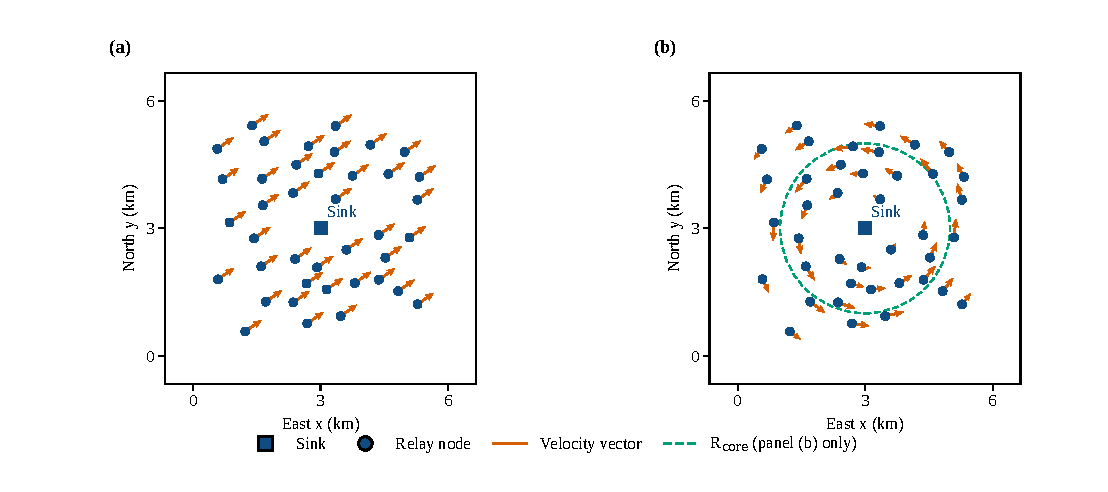
\includegraphics[width=\textwidth]{elqtp_figs/fig2_mobility_fields}
\caption{Velocity fields, $N=40$. (a)~Uniform current, $2\,\mathrm{m/s}$.
(b)~Rankine eddy, $R_{\mathrm{core}}=2000\,\mathrm{m}$.}
\label{fig:mobility_fields}
\end{figure*}

All four protocols share the constants of
Table~\ref{tab:sim_params}: $N=40$ relays in the
$6\,\mathrm{km}\times 6\,\mathrm{km}\times 500\,\mathrm{m}$ column,
January WOA23/GEBCO/Bellhop cell of
Section~\ref{sec:prelim:urick}, $\mathrm{SL}=175\,\mathrm{dB}$,
$R_b=1000\,\mathrm{bit/s}$, $l=400\,\mathrm{bit}$, $M=2$,
$\mathrm{SNR}_{\mathrm{th}}=8.68\,\mathrm{dB}$,
$r_{\mathrm{range}}=5125\,\mathrm{m}$, $E_{\mathrm{ini}}=10000\,\mathrm{J}$,
$\alpha=0.9$, $\gamma=0.8$, and SNR-threshold reception with no
modeled contention.
A node that leaves the area is removed.
Mobile runs use $T_{\mathrm{sim}}=600\,\mathrm{s}$ and
five independent random seeds.
The validated E-LQTP point is the event trigger on and
$\beta_1=\beta_2=0$.
Fixed-Periodic uses the same reward weights and
$T_{\mathrm{ctrl}}=5\,\mathrm{s}$.
That interval is one end-to-end delay of the $v=2\,\mathrm{m/s}$
mesh ($T_{\mathrm{e2e}}\approx 4.4\,\mathrm{s}$; one-hop flight
$\approx 2.0\,\mathrm{s}$ on the Scenario~III $\beta$ sweep).
It is a single, drift-independent budget against which an
event-triggered scheme can be cheaper or more expensive; it is
not claimed to be the optimal periodic timer, and it is the same
class of timer used to rebuild STGR's spatial-temporal graph
\cite{xu2025stgr} and to refresh QTAR and SAQR neighbor state
\cite{nandyala2023qtar,zhang2025saqr}.

% Drop-in for Section IV-A. Values from the campaign in Table I.
% Single-column: short two-column parameter list.

\begin{table}[!t]
\caption{Shared simulation parameters. E-LQTP-only knobs are marked.}
\label{tab:sim_params}
\centering
\scriptsize
\resizebox{\columnwidth}{!}{%
\begin{tabular}{lc}
\hline
Parameter & Value \\
\hline
Volume / $N$ / seeds & $6\,\mathrm{km}\times 6\,\mathrm{km}\times 500\,\mathrm{m}$ / $40$ / five \\
Site / season & $20.125^\circ\mathrm{N}$, $124.125^\circ\mathrm{E}$, January \\
Seafloor / carrier / band & $5524\,\mathrm{m}$ / $24\,\mathrm{kHz}$ / $2\,\mathrm{kHz}$ \\
$\mathrm{SL}$ / $\mathrm{DI}$ / $\mathrm{SNR}_{\mathrm{th}}$ & $175\,\mathrm{dB}$ / $0\,\mathrm{dB}$ / $8.68\,\mathrm{dB}$ \\
$R_b$ / $l$ / $M$ & $1000\,\mathrm{bit/s}$ / $400\,\mathrm{bit}$ / $2$ \\
$r_{\mathrm{range}}$ / $E_{\mathrm{ini}}$ & $5125\,\mathrm{m}$ / $10000\,\mathrm{J}$ \\
Efficiency / $P_{\mathrm{rx}}$ / BER floor & $0.5$ / $0.1\,\mathrm{W}$ / $10^{-9}$ \\
Data interval / $T_{\mathrm{sim}}$ / $dt$ & $30\,\mathrm{s}$ / $600\,\mathrm{s}$ / $1\,\mathrm{s}$ \\
$\alpha$ / $\gamma$ / reception / envelope & $0.9$ / $0.8$ / SNR gate / leave-area nodes removed \\
$\varepsilon_0$ / $s_{\mathrm{cap}}$ / $\lambda$ & $2.0\,\mathrm{dB}$ / $2.0\,\mathrm{dB}$ / $1.0$ \\
$W$ / $W_{\mathrm{mp}}$ / $\rho$ / $T_{\mathrm{ctrl}}$ / $(\beta_1,\beta_2)$ & $5$ / $3$ / $0.6$ / $5\,\mathrm{s}$ / $(0,0)$ \\
\hline
\end{tabular}}
\end{table}


Fig.~\ref{fig:mobility_fields} is the velocity field of the two
mobile scenarios on the same $N=40$ placement and the same fixed
sink.
Panel~(a) is shared current (Scenario~II): every relay has the same
horizontal velocity, so the true AUV--AUV range rate is identically
zero.
The filter does not start from that velocity.
Section~\ref{sec:design:kin} initializes the neighbor-velocity hold
at zero, and the hold takes the true value only after
$\mathrm{Broadcast}_k=1$.
Panel~(b) is the Rankine eddy (Scenario~III): arrow length scales
with local tangential speed, solid-body inside $R_{\mathrm{core}}$
and $1/r$ outside.
The figure's $1/r$ decay is the classical Rankine sketch; the
simulation itself uses the speed cap of \eqref{eq:rankine}.

Three scenarios are reported.
Scenario~I is the stationary identity of
Section~\ref{sec:eval:s1} ($T_{\mathrm{sim}}=1600\,\mathrm{s}$,
EKF not ticked, trigger off) and is a reproduction check, not a
primary mobility result.
Scenario~II sweeps $\|v_{\mathrm{drift}}\|$ at
$0.5$, $1.0$, $2.0$, $3.0$, and $3.5\,\mathrm{m/s}$.
Scenario~III uses $V_{\mathrm{eddy}}=2\,\mathrm{m/s}$ and
$R_{\mathrm{core}}=2000\,\mathrm{m}$.

\subsection{Metrics}
\label{sec:eval:metrics}
Packet-delivery ratio (PDR) is $N_{\mathrm{succ}}/N_{\mathrm{gen}}$
on packets whose source is still live.
End-to-end delay $T_{\mathrm{e2e}}$ and hop count are means over
successful deliveries.
Energy per bit $E_{\mathrm{bit}}$ follows LQARP's Eq.~45 on
\emph{data} transmissions only \cite{liu2026lqarp}.
Each data packet of $l=400\,\mathrm{bit}$ at
$R_b=1000\,\mathrm{bit/s}$ has airtime $0.4\,\mathrm{s}$.
Radiated acoustic power from $\mathrm{SL}=175\,\mathrm{dB}$ re
$1\,\mu\mathrm{Pa}@1\,\mathrm{m}$ is
$P_{\mathrm{ac}}=10^{(\mathrm{SL}-170.8)/10}=2.630\,\mathrm{W}$;
with projector efficiency $0.5$ the electrical transmit energy is
$E_{\mathrm{tx}}=2.104\,\mathrm{J}$ and the receive energy on a
successful decode is $E_{\mathrm{rx}}=0.040\,\mathrm{J}$.
Idle listening is not modelled, so $E_{\mathrm{bit}}$ measures
forwarding work, not modem duty cycle.

A dedicated HELLO uses the same $l=400\,\mathrm{bit}$ as a data
packet.
LQARP and RLOR-inspired emit no dedicated control frames, so their
$O_{\mathrm{ctrl}}$ is identically zero.
Section~\ref{sec:design:pkt} records that zero as an empty
control-byte count on the shared live pose.
E-LQTP and Fixed-Periodic add HELLO bytes on top of the same
data plane, whose energy is already inside $E_{\mathrm{bit}}$.
Because HELLO length equals $l$, control transmit power is the
linear image of $O_{\mathrm{ctrl}}$:
\begin{equation}
\label{eq:pctrl}
P_{\mathrm{ctrl}}
= \frac{O_{\mathrm{ctrl}}}{l/8}\,E_{\mathrm{tx}}
= O_{\mathrm{ctrl}}\times 4.208\times 10^{-2}\,\mathrm{W\cdot s/byte}.
\end{equation}
At the reported operating points this is $5.69\,\mathrm{W}$
network-wide under Scenario~II ($135.1\,\mathrm{byte/s}$) and
$8.88\,\mathrm{W}$ under Scenario~III ($211.0\,\mathrm{byte/s}$),
against a drift-independent Fixed-Periodic budget of
$17.40\,\mathrm{W}$ ($413.42\,\mathrm{byte/s}$, $41$ transmitters
$\times$ $121$ grid instants on $[0,600]\,\mathrm{s}$).
The joule ratios are therefore the same $0.33\times$ and
$0.51\times$ already reported in bytes per second.

The ratio of means that adds the mean HELLO transmit energy,
at $E_{\mathrm{tx}}=2.104\,\mathrm{J}$, to the mean data-plane
energy and divides by the mean number of delivered bits would
raise Scenario~II $E_{\mathrm{bit}}$ from $1.156\times 10^{-2}$
to $2.342\times 10^{-2}\,\mathrm{J/bit}$ for E-LQTP and to
$4.784\times 10^{-2}\,\mathrm{J/bit}$ for Fixed-Periodic.
LQARP would remain at $1.156\times 10^{-2}$ because it sends no
dedicated control frames.
We keep the LQARP definition of $E_{\mathrm{bit}}$ in the
protocol-comparison tables so the data-plane columns remain
comparable to the parent paper, and we report HELLO cost as
$O_{\mathrm{ctrl}}$ (and the $P_{\mathrm{ctrl}}$ conversion above).

First-fire is the fraction of live AUV--AUV pairs that experience
at least one rising-edge HELLO.
VOID counts empty-candidate drops.
Node-exit packet losses count packets whose forwarding node has
left the Bellhop envelope; they are recorded separately from
SNR-reception failures.
$n_{\mathrm{exit}}$ counts relays that leave the valid envelope.
Envelope attrition is a geometry fact, not a protocol difference.
Under Scenario~II the mean number of relays that exit by
$T_{\mathrm{sim}}$ is $1.8$, $4.4$, $9.4$, $14.4$, and $16.0$ of
$40$ at $0.5$, $1.0$, $2.0$, $3.0$, and $3.5\,\mathrm{m/s}$.
PDR in Table~\ref{tab:s2_drift} is therefore computed on a
shrinking live set; LQARP and E-LQTP lose the same nodes.

\subsection{Scenario I: Stationary Identity}
\label{sec:eval:s1}
Scenario~I freezes every node
($v_{\mathrm{cmd}}=v_{\mathrm{drift}}=0$)
for $T_{\mathrm{sim}}=1600\,\mathrm{s}$ and $N_{\mathrm{gen}}=2160$
at $N=40$.
E-LQTP is run in the identity configuration (trigger off,
$\varepsilon_0$ huge, EKF not ticked) so that any departure from
LQARP would be a code defect rather than a mobility effect
\cite{liu2026lqarp}.
Table~\ref{tab:s1_identity} reports the five-seed means.
LQARP and identity E-LQTP are bit-identical on every seed: PDR
$1.000$, hops $1.530\pm 0.068$, delay $3.078\pm 0.071\,\mathrm{s}$,
$E_{\mathrm{bit}}=8.20\pm 0.37\times 10^{-3}\,\mathrm{J/bit}$,
$O_{\mathrm{ctrl}}=0$, VOID $=0$.
Fixed-Periodic records $442.03\,\mathrm{byte/s}$ on this frozen
field.
A nominal budget of one $400$-bit HELLO from each of $41$ nodes
every $5\,\mathrm{s}$ is $410\,\mathrm{byte/s}$.
The recorded stationary rate exceeds that budget.
The mobile comparison in Section~\ref{sec:eval:metrics} uses the
exact grid $413.42\,\mathrm{byte/s}$ ($41$ transmitters $\times$
$121$ instants on $[0,600]\,\mathrm{s}$).
A timer still spends that control traffic on a field that cannot
change, the same class of waste a timer-rebuilt STG or a periodic
QTAR HELLO incurs on a frozen mesh
\cite{xu2025stgr,nandyala2023qtar}.
RLOR-inspired always takes the one-hop sink path
($\mathrm{hops}=1.000$) because it drops $N_{\mathrm{depth}}$ and
forwards $\arg\max P_{\mathrm{succ}}$; that is the opportunistic
construction surveyed in \cite{jiang2023orsurvey}, not a routing
win claimed against LQARP.
PDR saturates for all four protocols, which is the intended ceiling
of a stationary, range-rich column, not a primary comparison.

% Scenario I stationary identity. Single-column: four short rows.

\begin{table}[!t]
\caption{Scenario~I identity ($N=40$, $T_{\mathrm{sim}}=1600\,\mathrm{s}$,
five seeds). E-LQTP trigger off; PDR $=1.000$, VOID $=0$.}
\label{tab:s1_identity}
\centering
\scriptsize
\resizebox{\columnwidth}{!}{%
\begin{tabular}{lcccc}
\hline
Protocol & Hops & $T_{\mathrm{e2e}}$ (s) & $E_{\mathrm{bit}}$ & $O_{\mathrm{ctrl}}$ \\
\hline
LQARP & $1.530\pm 0.068$ & $3.078\pm 0.071$ & $8.20\pm 0.37\times 10^{-3}$ & $0$ \\
E-LQTP & $1.530\pm 0.068$ & $3.078\pm 0.071$ & $8.20\pm 0.37\times 10^{-3}$ & $0$ \\
RLOR-insp. & $1.000\pm 0$ & $1.887\pm 0.108$ & $5.36\times 10^{-3}$ & $0$ \\
Periodic & $1.546\pm 0.039$ & $3.119\pm 0.188$ & $8.29\pm 0.21\times 10^{-3}$ & $442.03$ \\
\hline
\end{tabular}}
\end{table}


\subsection{Scenario II: Uniform Current Drift}
\label{sec:eval:s2}
\begin{figure*}[!t]
\centering
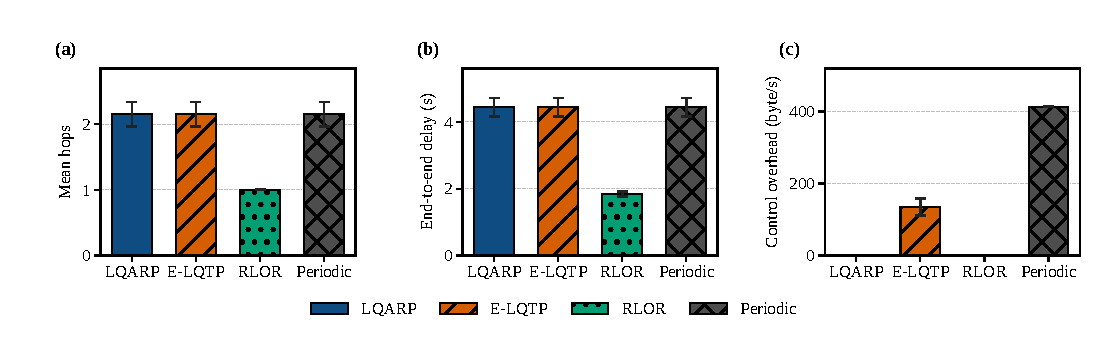
\includegraphics[width=\textwidth]{elqtp_figs/fig3_scenario2_protocols}
\caption{Scenario~II at $2\,\mathrm{m/s}$: hops, delay, and
$O_{\mathrm{ctrl}}$. Error bars are the five-seed sample standard
deviation.}
\label{fig:scenario2_protocols}
\end{figure*}

\begin{figure*}[!t]
\centering
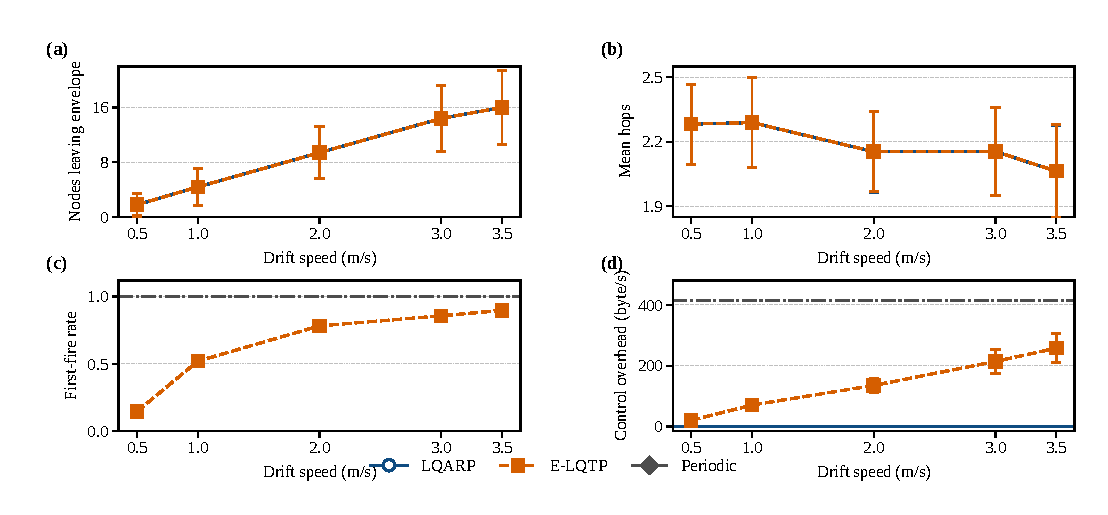
\includegraphics[width=\textwidth]{elqtp_figs/fig4_scenario2_drift}
\caption{Scenario~II versus drift: exits, hops, first-fire, and
$O_{\mathrm{ctrl}}$. Error bars are the five-seed sample standard
deviation.}
\label{fig:scenario2_drift}
\end{figure*}

Table~\ref{tab:s2_protocols} and Fig.~\ref{fig:scenario2_protocols}
compare the four protocols at the reported midpoint
$\|v_{\mathrm{drift}}\|=2\,\mathrm{m/s}$.
E-LQTP reproduces LQARP's data plane---PDR $0.9992\pm 0.0019$,
hops $2.154$ versus $2.153$, delay $4.439\,\mathrm{s}$ versus
$4.438\,\mathrm{s}$, identical $E_{\mathrm{bit}}$ at the printed
precision, identical node-exit packet losses
($0.60\pm 1.34$), VOID $=0$---and cuts control traffic from the
analytic $413.42\,\mathrm{byte/s}$ grid to
$135\pm 23\,\mathrm{byte/s}$ ($0.33\times$, never above $163$).
First-fire is $0.782\pm 0.042$.
By the definition in Section~\ref{sec:eval:metrics} this is the
fraction of live AUV--AUV pairs that record at least one rising
edge.
The true AUV--AUV range rate is zero once both velocities are known.
Those pairs still fire because the velocity hold begins at zero, so
the forecast initially integrates the observer's own drift.
After the hold is written, the constant-velocity model matches the
shared current.
Links to the fixed sink retain a nonzero range rate after that
write.
Fixed-Periodic at $\beta_1=\beta_2=0$ is LQARP's data plane plus
that flat HELLO grid on the shared live pose of
Section~\ref{sec:design:pkt}, which isolates the timer from the
reward.
RLOR-inspired again sits at one hop ($T_{\mathrm{e2e}}=1.845\,\mathrm{s}$)
because the sink remains in $N_{\mathrm{SNR}}$ for live relays; it
has no dedicated control plane.

% Scenario II four-protocol headline. Wide 7-col: stay table*.

\begin{table*}[!t]
\caption{Scenario~II at $2\,\mathrm{m/s}$ ($N=40$, five seeds,
$\beta_1=\beta_2=0$). Entries with $\pm$ are the sample standard
deviation. VOID $=0$.}
\label{tab:s2_protocols}
\centering
\small
\begin{tabular}{lcccccc}
\hline
Protocol & PDR & $T_{\mathrm{e2e}}$ (s) & $E_{\mathrm{bit}}$
  & $O_{\mathrm{ctrl}}$ & Hops & First-fire \\
\hline
LQARP & $0.9992\pm 0.0019$ & $4.438\pm 0.277$ & $1.156\pm 0.100\times 10^{-2}$
  & $0$ & $2.153\pm 0.187$ & --- \\
E-LQTP & $0.9992\pm 0.0019$ & $4.439\pm 0.277$ & $1.156\pm 0.100\times 10^{-2}$
  & $135\pm 23$ & $2.154\pm 0.187$ & $0.782\pm 0.042$ \\
RLOR-insp. & $1.0000\pm 0$ & $1.845\pm 0.074$ & $5.362\times 10^{-3}$
  & $0$ & $1.000\pm 0.001$ & --- \\
Periodic & $0.9992\pm 0.0019$ & $4.438\pm 0.277$ & $1.156\pm 0.100\times 10^{-2}$
  & $413.42$ & $2.153\pm 0.187$ & $1.000$ \\
\hline
\end{tabular}
\end{table*}


Table~\ref{tab:s2_drift} and Fig.~\ref{fig:scenario2_drift} sweep
drift magnitude.
The hop ratio E-LQTP/LQARP is $1.000\times$ at every $v$.
PDR, delay, and node-exit packet losses match LQARP at every $v$.
Energy per data bit agrees with LQARP through the digits of
Table~\ref{tab:s2_protocols}; across the sweep the largest
relative difference is below $3\times 10^{-4}$.
$O_{\mathrm{ctrl}}$ over the periodic $413.4\,\mathrm{byte/s}$ is
$0.05\times$, $0.17\times$, $0.33\times$, $0.52\times$, and
$0.62\times$ at $0.5$, $1$, $2$, $3$, and $3.5\,\mathrm{m/s}$.
First-fire rises with drift, $15\%\to 52\%\to 78\%\to 86\%\to 90\%$.
Panel~(a) of Fig.~\ref{fig:scenario2_drift} is envelope exits, not
PDR: the two protocols lose the same relays.
Even at $3.5\,\mathrm{m/s}$ E-LQTP stays under the periodic budget.

% Scenario II drift sweep. Wide 7-col: stay table*.

\begin{table*}[!t]
\caption{Scenario~II versus drift (LQARP vs.\ E-LQTP; five seeds,
$\beta_1=\beta_2=0$). Hop ratio $1.000\times$ at every $v$.}
\label{tab:s2_drift}
\centering
\small
\begin{tabular}{ccccccc}
\hline
$v$ (m/s) & Protocol & PDR & $T_{\mathrm{e2e}}$ (s) & $O_{\mathrm{ctrl}}$
  & Hops & First-fire \\
\hline
$0.5$ & LQARP & $1.000$ & $4.776\pm 0.403$ & $0$ & $2.282\pm 0.186$ & --- \\
$0.5$ & E-LQTP & $1.000$ & $4.776\pm 0.403$ & $20.2\pm 4.2$ & $2.282\pm 0.186$ & $0.146\pm 0.021$ \\
$1.0$ & LQARP & $0.9995\pm 0.0012$ & $4.752\pm 0.377$ & $0$ & $2.289\pm 0.208$ & --- \\
$1.0$ & E-LQTP & $0.9995\pm 0.0012$ & $4.752\pm 0.377$ & $70.7\pm 6.2$ & $2.289\pm 0.208$ & $0.520\pm 0.031$ \\
$2.0$ & LQARP & $0.9992\pm 0.0019$ & $4.438\pm 0.277$ & $0$ & $2.153\pm 0.187$ & --- \\
$2.0$ & E-LQTP & $0.9992\pm 0.0019$ & $4.439\pm 0.277$ & $135.1\pm 23.1$ & $2.154\pm 0.187$ & $0.782\pm 0.042$ \\
$3.0$ & LQARP & $1.000$ & $4.431\pm 0.333$ & $0$ & $2.154\pm 0.203$ & --- \\
$3.0$ & E-LQTP & $1.000$ & $4.433\pm 0.331$ & $213.8\pm 39.1$ & $2.155\pm 0.203$ & $0.857\pm 0.034$ \\
$3.5$ & LQARP & $1.000$ & $4.200\pm 0.393$ & $0$ & $2.063\pm 0.215$ & --- \\
$3.5$ & E-LQTP & $1.000$ & $4.200\pm 0.393$ & $257.7\pm 46.9$ & $2.063\pm 0.215$ & $0.897\pm 0.028$ \\
\hline
\end{tabular}
\end{table*}


\subsection{Scenario III: Rankine Eddy}
\label{sec:eval:s3}
\begin{figure*}[!t]
\centering
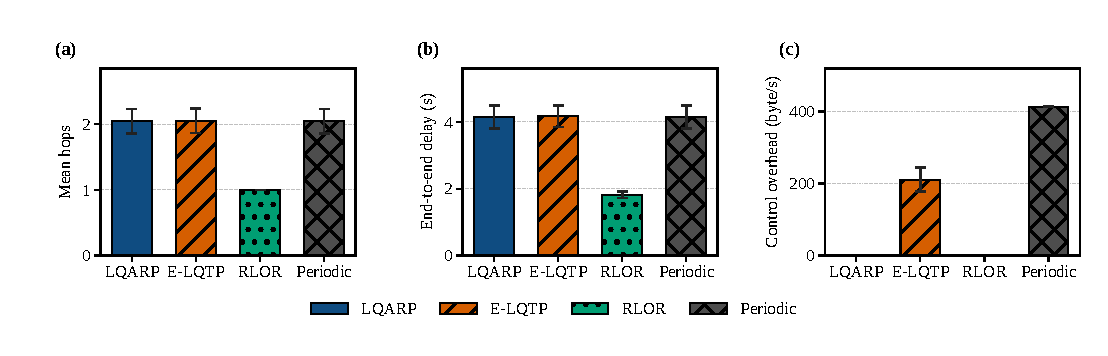
\includegraphics[width=\textwidth]{elqtp_figs/fig5_scenario3_protocols}
\caption{Scenario~III at $V_{\mathrm{eddy}}=2\,\mathrm{m/s}$: hops,
delay, and $O_{\mathrm{ctrl}}$. Error bars are the five-seed sample
standard deviation.}
\label{fig:scenario3_protocols}
\end{figure*}

Table~\ref{tab:s3_protocols} and Fig.~\ref{fig:scenario3_protocols}
repeat the four-protocol comparison under the eddy.
E-LQTP again matches LQARP (PDR $0.9989\pm 0.0018$, hops
$2.050/2.046=1.002\times$, delay $4.167\,\mathrm{s}$ versus
$4.146\,\mathrm{s}$, energy $1.101\times 10^{-2}$ versus
$1.099\times 10^{-2}\,\mathrm{J/bit}$, node-exit packet losses
$0.80\pm 1.30$ for both, VOID $=0$) at
$211\pm 34\,\mathrm{byte/s}$ versus
$413.42\,\mathrm{byte/s}$ ($0.51\times$).
First-fire is $0.708\pm 0.059$; mean exits are $6.40\pm 1.14$ of
$40$, identical across protocols.
The leftover $0.2\%$ hop difference is $N_{\mathrm{stab}}$ with the
trigger on.
A separate five-seed run with $\beta_1=\beta_2=1$ together, outside
the one-at-a-time sweep of Table~\ref{tab:beta_sweep}, produced
$3.250\pm 0.141$ hops against LQARP's $2.046\pm 0.187$
($1.59\times$).
That increase is the scale-mismatched $c_{\mathrm{pred}}$ at an
$O(1)$ weight.
The point is reported only as a diagnostic.

% Scenario III four-protocol headline. Wide 7-col: stay table*.

\begin{table*}[!t]
\caption{Scenario~III at $V_{\mathrm{eddy}}=2\,\mathrm{m/s}$
($N=40$, five seeds, $\beta_1=\beta_2=0$). Entries with $\pm$ are
the sample standard deviation. VOID $=0$.}
\label{tab:s3_protocols}
\centering
\small
\begin{tabular}{lcccccc}
\hline
Protocol & PDR & $T_{\mathrm{e2e}}$ (s) & $E_{\mathrm{bit}}$
  & $O_{\mathrm{ctrl}}$ & Hops & First-fire \\
\hline
LQARP & $0.9989\pm 0.0018$ & $4.146\pm 0.348$ & $1.099\pm 0.098\times 10^{-2}$
  & $0$ & $2.046\pm 0.187$ & --- \\
E-LQTP & $0.9989\pm 0.0018$ & $4.167\pm 0.318$ & $1.101\pm 0.097\times 10^{-2}$
  & $211\pm 34$ & $2.050\pm 0.186$ & $0.708\pm 0.059$ \\
RLOR-insp. & $1.0000\pm 0$ & $1.814\pm 0.093$ & $5.361\times 10^{-3}$
  & $0$ & $1.000\pm 0$ & --- \\
Periodic & $0.9989\pm 0.0018$ & $4.146\pm 0.348$ & $1.099\pm 0.098\times 10^{-2}$
  & $413.42$ & $2.046\pm 0.187$ & $1.000$ \\
\hline
\end{tabular}
\end{table*}


The pair-level trace of Fig.~\ref{fig:trigger_trace} is
Scenario~III pair $(1,2)$.
The three rising edges at $348$, $483$, and $512\,\mathrm{s}$ are
that pair's HELLOs, not the network-wide count.
The network-wide count is $O_{\mathrm{ctrl}}$: the forecast track
is allowed to drift, and a HELLO is charged only on a rising edge
\cite{li2026dse,priel2023consensus}.

\subsection{Reward Ablation}
\label{sec:eval:beta}
\begin{figure*}[!t]
\centering
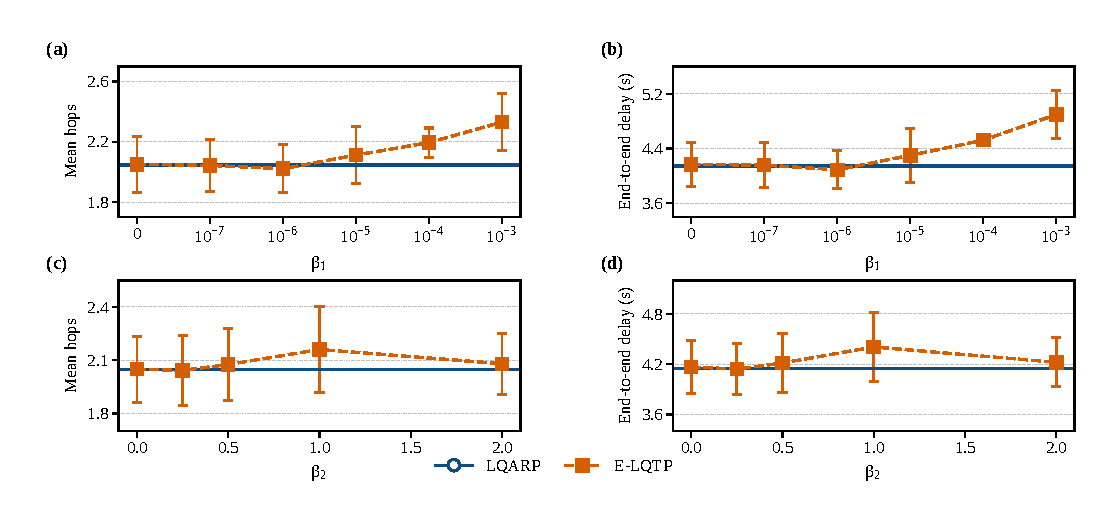
\includegraphics[width=\textwidth]{elqtp_figs/fig6_reward_ablation}
\caption{Scenario~III reward sweep. Solid line: LQARP. Error bars
are the five-seed sample standard deviation. No tested $\beta$
improves hops or delay.}
\label{fig:reward_ablation}
\end{figure*}

Table~\ref{tab:beta_sweep} and Fig.~\ref{fig:reward_ablation} sweep
$\beta_1$ at $\beta_2=0$ and $\beta_2$ at $\beta_1=0$ on
Scenario~III.
At $\beta_1=10^{-6}$ mean hops fall to $2.021\pm 0.158$ against
LQARP's $2.046\pm 0.187$ ($0.988\times$); that dip sits inside
LQARP's between-seed band and is not read as a routing gain.
Once $\beta_1$ leaves the blend-scale range, hops, delay, and
energy rise together, reaching $1.14\times$ hops and
$1.18\times$ delay at $\beta_1=10^{-3}$.
The $\beta_2$ column stays within $0.998\times$--$1.056\times$
LQARP hops with no monotonic trend.
No tested weight improves hops, delay, or energy relative to
LQARP's between-seed band.
A Scenario~II-specific $\beta_2$ sweep against the sustained
AUV--sink range-rate of uniform drift remains future work.
The validated operating point is therefore $\beta_1=\beta_2=0$:
the control-plane gain is the event trigger, and the reward
modifiers are a documented negative result.

% Scenario III reward sweep. Five columns: single-column table.

\begin{table}[!t]
\caption{Scenario~III $\beta$ sweeps (five seeds). No tested weight
beats LQARP's hop or delay band.}
\label{tab:beta_sweep}
\centering
\scriptsize
\resizebox{\columnwidth}{!}{%
\begin{tabular}{lcccc}
\hline
Weight & PDR & $T_{\mathrm{e2e}}$ (s) & $E_{\mathrm{bit}}$ & Hops \\
\hline
LQARP & $0.9989\pm 0.0018$ & $4.146\pm 0.348$ & $1.099\pm 0.098\times 10^{-2}$ & $2.046\pm 0.187$ \\
\hline
\multicolumn{5}{l}{$\beta_1$ sweep ($\beta_2=0$)} \\
$0$ & $0.9989\pm 0.0018$ & $4.167\pm 0.318$ & $1.101\pm 0.097\times 10^{-2}$ & $2.050\pm 0.186$ \\
$10^{-7}$ & $0.9986\pm 0.0017$ & $4.159\pm 0.324$ & $1.098\pm 0.092\times 10^{-2}$ & $2.043\pm 0.175$ \\
$10^{-6}$ & $1.0000\pm 0$ & $4.090\pm 0.279$ & $1.083\pm 0.085\times 10^{-2}$ & $2.021\pm 0.158$ \\
$10^{-5}$ & $1.0000\pm 0$ & $4.301\pm 0.399$ & $1.132\pm 0.103\times 10^{-2}$ & $2.111\pm 0.192$ \\
$10^{-4}$ & $0.9976\pm 0.0040$ & $4.523\pm 0.082$ & $1.185\pm 0.056\times 10^{-2}$ & $2.194\pm 0.097$ \\
$10^{-3}$ & $0.9980\pm 0.0027$ & $4.897\pm 0.351$ & $1.253\pm 0.099\times 10^{-2}$ & $2.330\pm 0.188$ \\
\hline
\multicolumn{5}{l}{$\beta_2$ sweep ($\beta_1=0$)} \\
$0$ & $0.9989\pm 0.0018$ & $4.167\pm 0.318$ & $1.101\pm 0.097\times 10^{-2}$ & $2.050\pm 0.186$ \\
$0.25$ & $0.9989\pm 0.0018$ & $4.140\pm 0.304$ & $1.097\pm 0.103\times 10^{-2}$ & $2.042\pm 0.197$ \\
$0.50$ & $0.9989\pm 0.0018$ & $4.214\pm 0.349$ & $1.115\pm 0.106\times 10^{-2}$ & $2.076\pm 0.204$ \\
$1.00$ & $0.9989\pm 0.0018$ & $4.405\pm 0.415$ & $1.160\pm 0.126\times 10^{-2}$ & $2.161\pm 0.240$ \\
$2.00$ & $0.9989\pm 0.0018$ & $4.221\pm 0.293$ & $1.117\pm 0.090\times 10^{-2}$ & $2.080\pm 0.171$ \\
\hline
\end{tabular}}
\end{table}


\subsection{Discussion Against Recent Journal Protocols}
\label{sec:eval:disc}
The primary claim is a control-plane claim, not a new data-plane
reward.
QTAR, SAQR, the hierarchical Q-learning cluster of Yuan
\emph{et~al.}, ADRP-DQL, CLORP, STGR, and SDN-QLTR all improve
forwarding by redesigning the Q-update or the candidate set, and
they keep neighbor state current on a timer
\cite{nandyala2023qtar,zhang2025saqr,yuan2023qhier,mohanraju2025adrp,liu2024clorP,xu2025stgr,li2024sdnqltr}.
E-LQTP leaves LQARP's reward untouched \cite{liu2026lqarp} and
charges a HELLO only when the forecast track diverges from the
per-tick channel query.
Scenario~II and Scenario~III match LQARP's hops and delay to three
figures because both routers read the same live pose and the
validated weights are $\beta_1=\beta_2=0$, while $O_{\mathrm{ctrl}}$
falls to $0.33\times$ and $0.51\times$ the $5\,\mathrm{s}$ grid used
as the periodic baseline in this campaign.
Those factors are the timing ablation under the shared pose of
Section~\ref{sec:design:pkt}.
QTAR, SAQR, and STGR are cited as members of that timer class
\cite{nandyala2023qtar,zhang2025saqr,xu2025stgr}.
They were not reimplemented on this site, so the factors above are
not a claim that their published overhead equals
$413.42\,\mathrm{byte/s}$.
QLAR is the design that already adapts a HELLO period, and it does
so from predicted link lifetime rather than from
\eqref{eq:etrigger} \cite{li2025qlar}.

Trust-aware and clustered opportunistic designs (He \emph{et~al.},
RCRP, FHOEEC, LSLPR) and the information-centric push/pull family
(push-hybrid UNDN, RECAR, Wang--Lu--Gao) likewise treat the beacon
as a security, void, or naming event
\cite{he2025trust,zhu2024rcrp,lee2025fho,tian2023lslpr,wang2024push,li2024recar,wang2025reliable,zhao2026trclor}.
None of those events is the forecast-versus-truth SNR residual of
Section~III, so their control traffic does not automatically
collapse when relative geometry is temporarily stable.
AUV collection and path-planning DQNs
\cite{wang2024lgdqn,liu2025mdqn,lu2025wper,nandyala2025isolated}
move the vehicle rather than the HELLO timer; they are complementary
to E-LQTP, not substitutes.
The same holds for acoustic--radio hybrid hops
\cite{jiang2023hybrid}, multi-objective and cross-layer schedules
\cite{yuan2024multiobj,yuan2024crosslayer}, MARV's value-of-information
split \cite{wang2024marv}, GMM--HMM--LSTM adaptation and trust
guidelines \cite{zhu2024gmmhmm,zhu2024trustcomst}, and the Zhoushan
multipath sea trial \cite{yuan2024multipath}: each changes the
forwarding objective or the physical path, not the HELLO cadence.

The event-triggered Kalman literature
\cite{li2026dse,priel2023consensus,sebastian2024eco,deng2023auto,zhong2024tsp,deng2024lcsys}
already showed that a predicted information pair can replace a
periodic sample.
E-LQTP reuses that idea for a routing HELLO on a per-tick Bellhop
query.
The $2\,\mathrm{dB}$ cap is this paper's choice, placed below the
LOON21 Kalman mean absolute errors $4.81$, $3.47$, and
$3.24\,\mathrm{dB}$ \cite{busacca2024snr}.
The $\beta$ ablation then shows that folding the same innovation
into $c_{\mathrm{pred}}$ and $c_{\mathrm{drift}}$ does not buy a
data-plane gain on this grid---a scoped negative result relative
to the reward-heavy Q-learning family above.

\FloatBarrier

\section{Conclusion}
\label{sec:conclusion}
\IEEEPARstart{T}{his} article addressed the control-plane cost of
keeping link-quality state accurate in a mobile underwater mesh.
E-LQTP adds a dual-track extended Kalman filter to LQARP so that a
HELLO fires only when a forecast that receives no measurement update
diverges from the per-tick channel query. With the trigger on and
$\beta_1=\beta_2=0$, E-LQTP matches LQARP's packet
delivery ratio, hop count, end-to-end delay, and energy per data
bit, while cutting control traffic to $0.33\times$ a
$5\,\mathrm{s}$ periodic grid under $2\,\mathrm{m/s}$ drift and
to $0.51\times$ under the Rankine eddy.
The campaign counts those control bytes in $O_{\mathrm{ctrl}}$.
Reception is the SNR gate of Section~\ref{sec:design:ns3}, and
HELLO energy is left out of residual energy, so the reported
saving is the byte count on the shared live pose.
The additive reward terms do not improve hops or delay; that
negative result is reported rather than tuned away, isolating the
gain to the event-triggered mechanism itself.

A relative-form $c_{\mathrm{pred}}$ and a Scenario~II-only
$\beta_2$ sweep against sustained AUV--sink range-rate remain
future work, together with a neighbor table that ages between
velocity copies and a non-ground-truth channel-estimation
pipeline for the staleness test.

\section*{Acknowledgment}
This work was supported in part by the China Postdoctoral Science
Foundation under Grant 2025M784399; in part by the Heilongjiang
Postdoctoral Fund under Grant LBH-Z25121; in part by the Fundamental
Research Funds for the Central Universities under Grant 3072026LJ0801;
in part by the ``Double First Class'' Discipline Collaborative
Innovation Achievement Project of Heilongjiang Province under Grant
LJGXCG2023-066; in part by the Major Scientific and Technological
Achievements Commercialization Project of Heilongjiang Province under
Grant ZC2024SH0024.


\bibliographystyle{IEEEtran}
\bibliography{refs}

\end{document}
